\begin{comment}
	\pagebreak
\end{comment}

\section{Fully Convolutional Neural Network}
\begin{comment}
	The main difference to classical CNN is that we don't want to only work with fixed sized images as input. 
	This limitation comes from the fully connected layers in the end.\\
\end{comment}

\textbf{Semantic segment.:} extract patch, run through cnn, classify\\
+ size independen, - only local context
\begin{comment}
	We extract each patch and run it through a CNN. 
	This let's us classify a pixel by it's local neighbourhood, but we loose the whole context of the pixel, as we are not looking at the whole image anymore.\\
	\textbf{Approach:} learn features of the input image (encoding), which is followed by a decoder who projects the learned features to the higher resolution pixel space.
	We get rid of the fully connected layer at the end of the network.\\
	
	\begin{Figure}
 		\centering
 		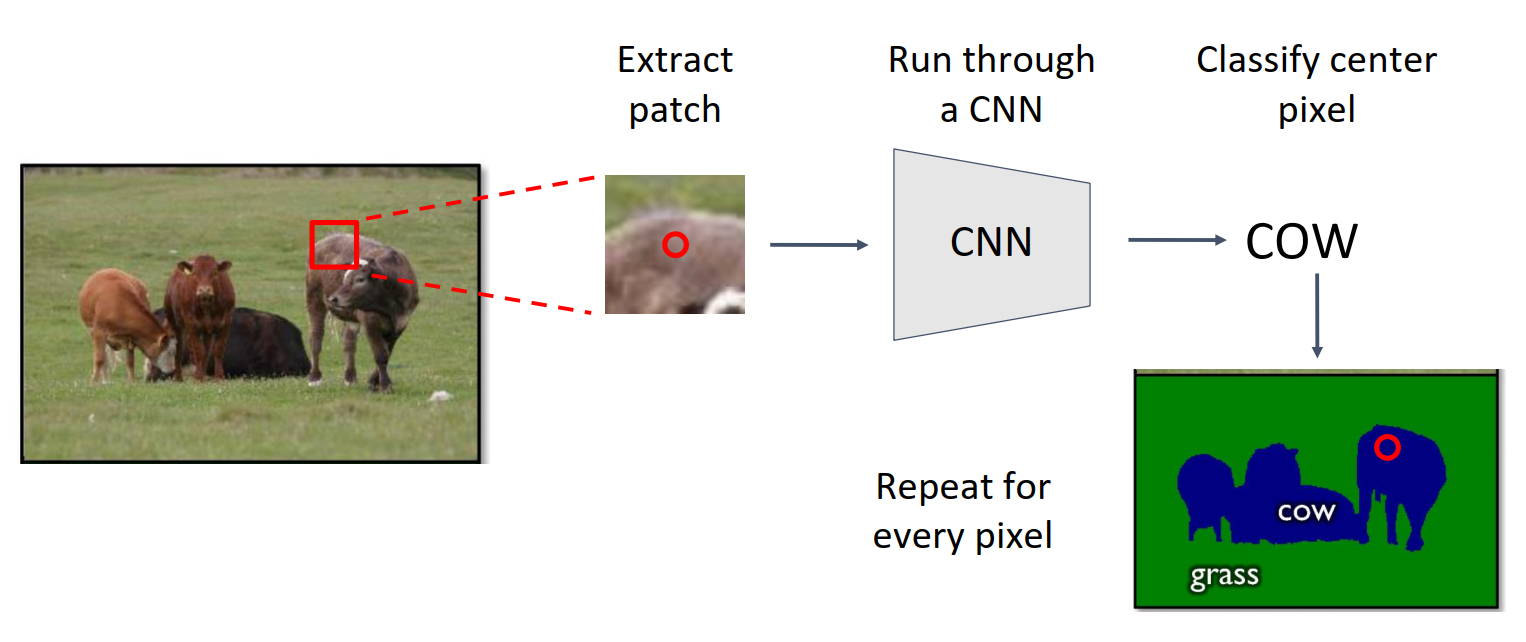
\includegraphics[width=\linewidth]{graphic/fcnn-semantic-segmentation-pipeline}
 		\captionof{figure}{Pixel-wise classification pipeline}
	\end{Figure}
\end{comment}

\textbf{Downsample:} pooling or strides, otherwise very expensive\\
\begin{comment}
	Downsampling helps with performance, as not the whole image is run through convolutions.
	But, it results in low resolution and fuzzy object boundaries.
	Newer architectures can mitigate this by copying the learned features from the downsampling stage into the upsampling stage.\\
	
	\begin{Figure}
 		\centering
 		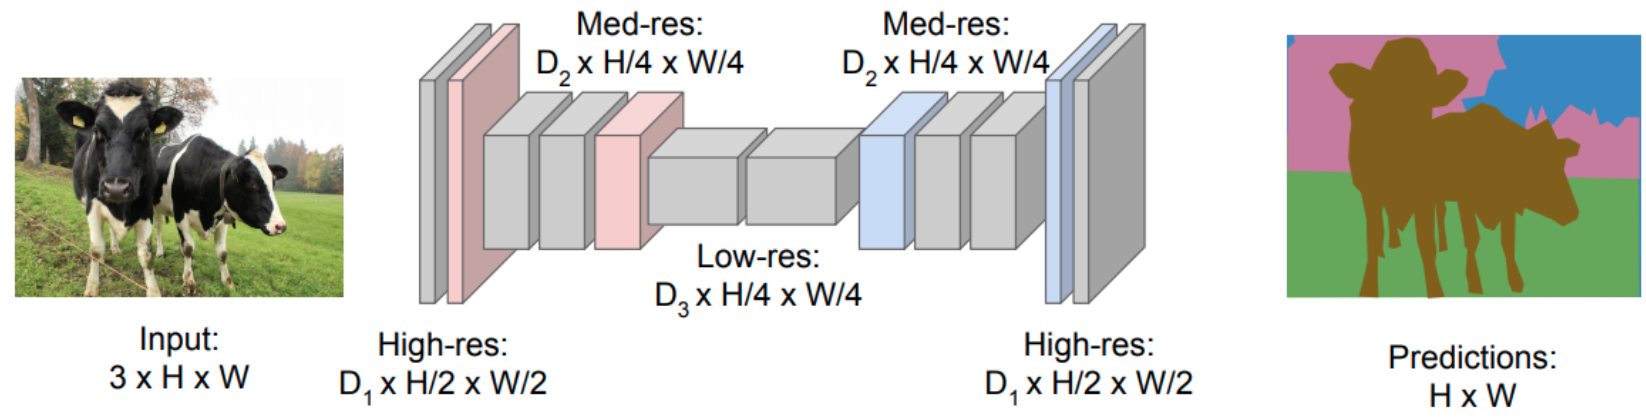
\includegraphics[width=\linewidth]{graphic/fcnn-low-res-mitigation}
 		\captionof{figure}{Downsample and than upsample to increase resolution again}
	\end{Figure}
\end{comment}

\textbf{Nearest Neighbor:} copy value to the whole output\\ 
\begin{comment}
	Upsampling can be seen as interpolation, increasing the resolution of the signal.\\
	
	\begin{Figure}
 		\centering
 		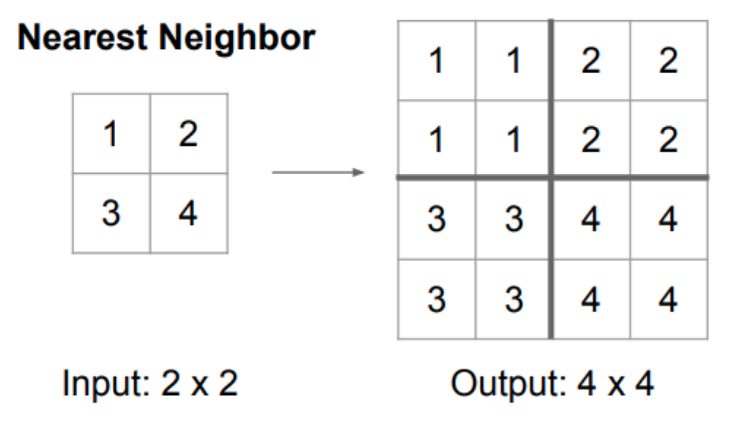
\includegraphics[width=\linewidth]{graphic/fcnn-nn-upsampling}
 		\captionof{figure}{Copy input pixel to all output pixels}
	\end{Figure}
\end{comment}

\textbf{Bed-of-nails:} zero all outputs but one copy of input\\
\begin{comment}
	\begin{Figure}
 		\centering
 		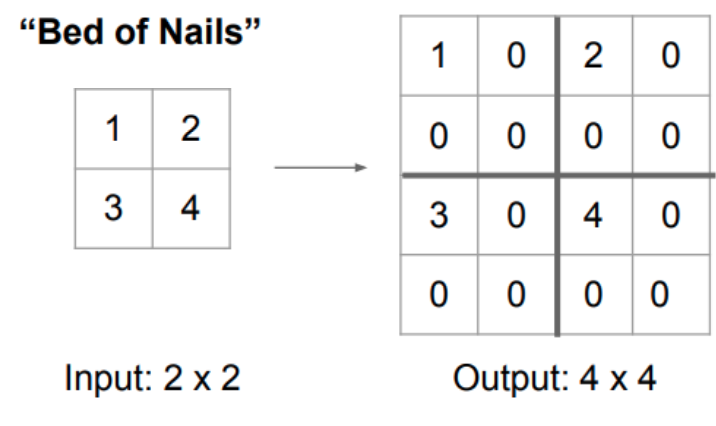
\includegraphics[width=\linewidth]{graphic/fcnn-bos-upsampling}
 		\captionof{figure}{Copy input pixel to one output pixels, rest zero}
	\end{Figure}
\end{comment}

\textbf{Max-unpooling:} remember max element from downsampling, use that in upsampling\\
\begin{comment}
	\begin{Figure}
 		\centering
 		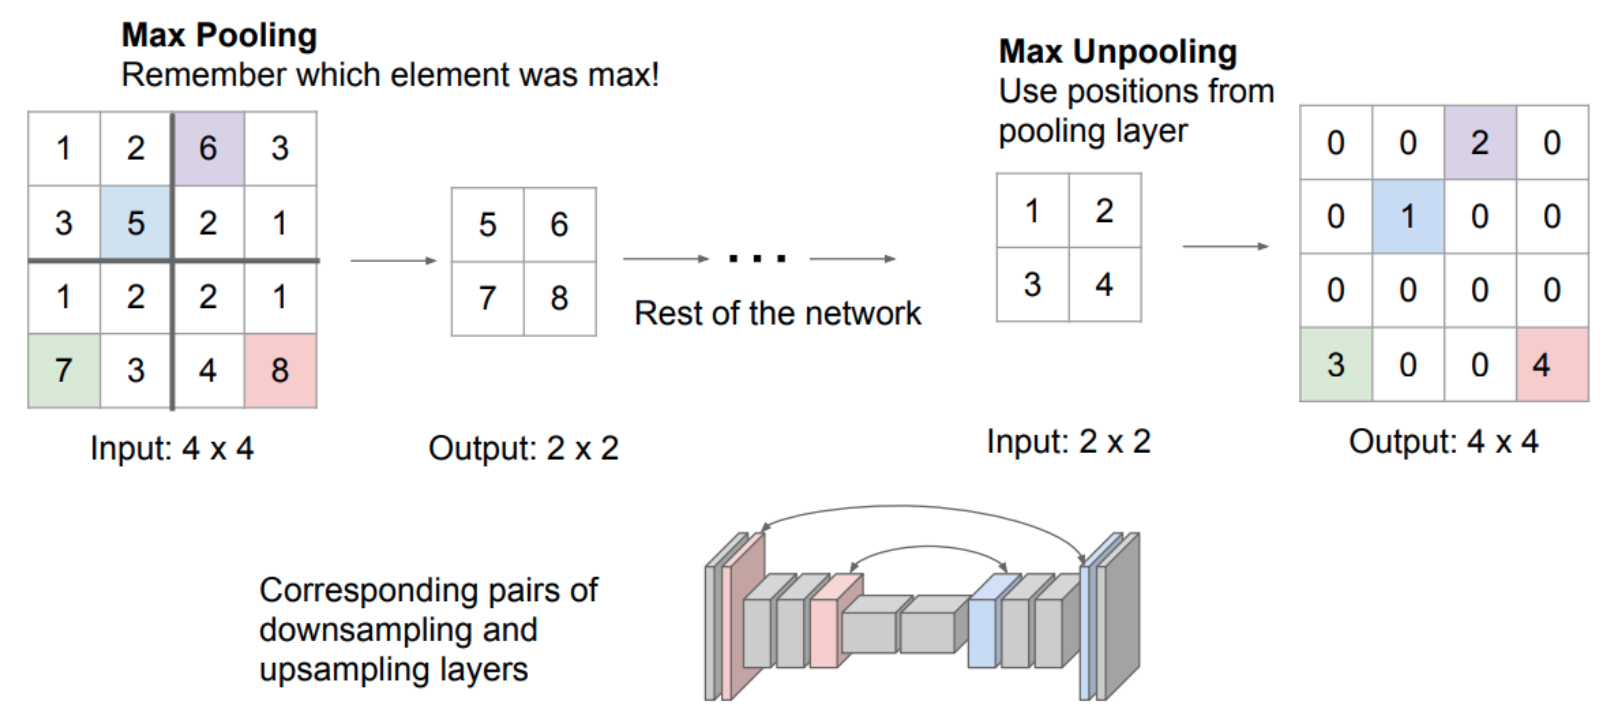
\includegraphics[width=\linewidth]{graphic/fcnn-max-unpooling-upsampling}
 		\captionof{figure}{Copy input pixel to location of the max pooling pixel}
	\end{Figure}
\end{comment}

\textbf{Learnable Upsampling:} input as weight, add up filters in output\\
\begin{comment}
	\begin{Figure}
 		\centering
 		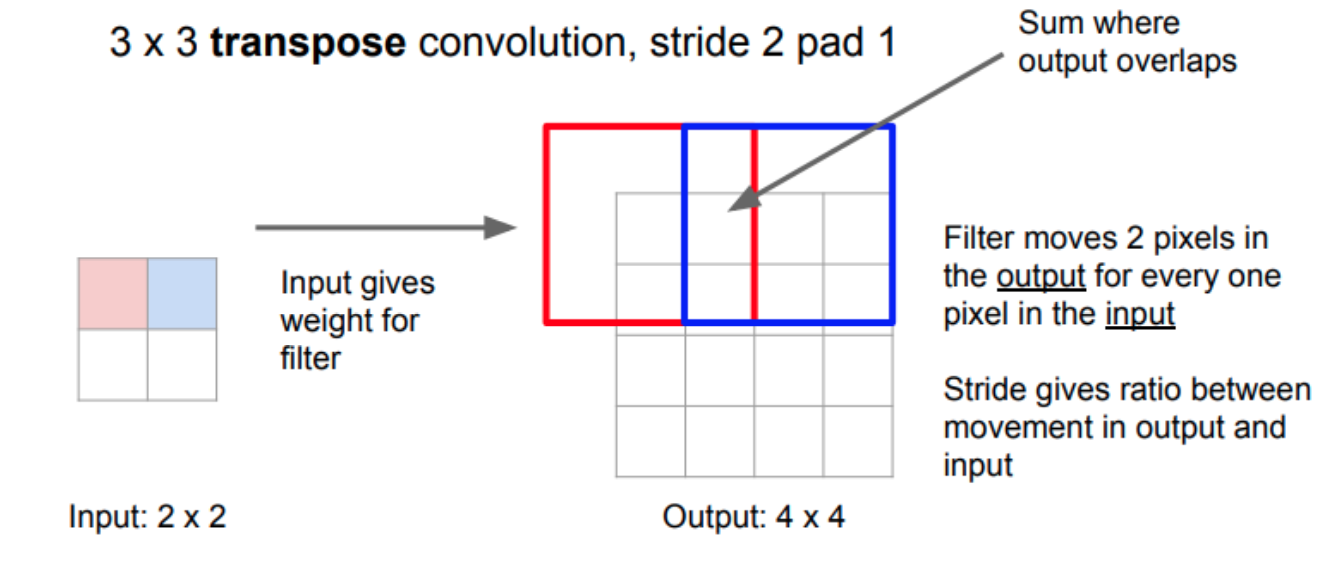
\includegraphics[width=\linewidth]{graphic/fcnn-transpose-convolution}
 		\captionof{figure}{Input pixel gives the weight for a filter}
	\end{Figure}
\end{comment}

\textbf{UNet:} copy early stage tensors to upsampling, combines local and global feature maps\\
\begin{comment}
	Main idea: combine global and local feature maps by copying corresponding tensors from earlier stages into later stages.\\
	Also, the downsampling information is pretty shallow, upsampling performance is improved when including "pre-downsamplin" information.\\

	\begin{Figure}
 		\centering
 		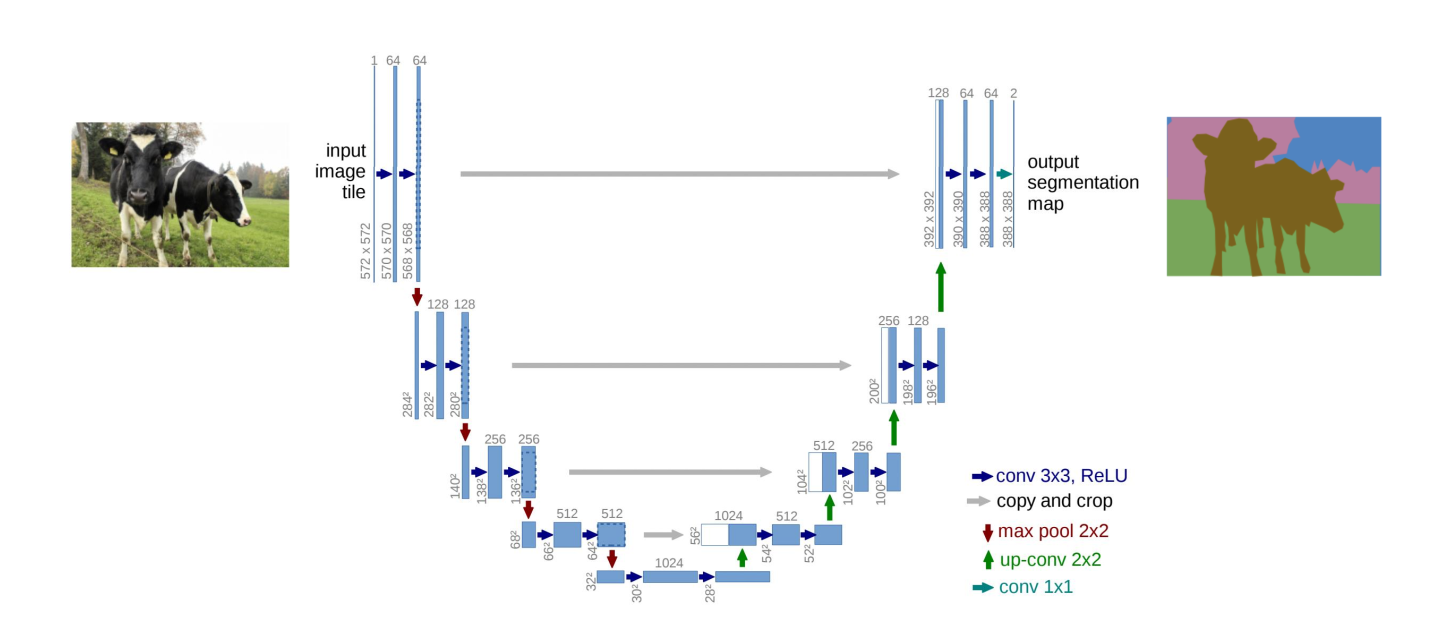
\includegraphics[width=\linewidth]{graphic/fcnn-unet}
 		\captionof{figure}{U-Net architecture}
	\end{Figure}
\end{comment}





